\documentclass{beamer}
\usepackage{stmaryrd}
\usepackage{bussproofs}
\usepackage{bbm}

\AtBeginSection[]{
    \begin{frame}{}
    \tableofcontents[currentsection]
    \end{frame}
}

\newlength{\layerwidth}
\setlength{\layerwidth}{.4\textwidth}
%\setlength{\parskip}{1em}

\newcommand{\kw}[1]{\texttt{#1}}
\newcommand{\ljg}[5]{{#2} \vdash^{#1}_{#3} {#4} : {#5}}
\newcommand{\jg}[4]{\ljg{}{#1}{#2}{#3}{#4}}
\newcommand{\module}[1]{\UnaryInfC{\framebox[\layerwidth]{#1}}}
\newcommand{\nonmodule}[1]{\UnaryInfC{\makebox[\layerwidth]{#1}}}
\newcommand{\layer}[1]{\RightLabel{\footnotesize #1}}

\title{Refinement-Based Game Semantics for \\ Certified Abstraction Layers}
\author{J\'er\'emie Koenig}

\begin{document}

\begin{frame}
\titlepage
\end{frame}

\section{Introduction}

\begin{frame}{Certified Abstraction Layers}
\small
\begin{tabular}{lcc}
\rule[-2em]{0pt}{4em}
Elementary proof &
\rule{0pt}{5ex}
\AxiomC{$\kw{CP}(L, R, \kappa, \sigma)$}
\UnaryInfC{$\jg{L}{R}{i \mapsto \kappa}{i \mapsto \sigma}$}
\DisplayProof &
\begin{minipage}[c]{.1\textwidth}
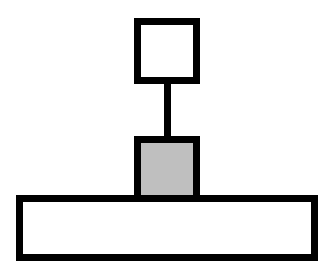
\includegraphics[scale=.15]{element}
\end{minipage} \\
\rule[-2em]{0pt}{4em}
Horizontal composition &
\rule{0pt}{5ex}
\AxiomC{$\jg{L}{R}{M_1}{L_1}$}
\AxiomC{$\jg{L}{R}{M_2}{L_2}$}
\BinaryInfC{$\jg{L}{R}{M_1 \oplus M_2}{L_1 \oplus L_2}$}
\DisplayProof &
\begin{minipage}[c]{.1\textwidth}
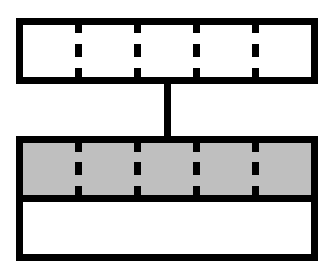
\includegraphics[scale=.15]{hcomp}
\end{minipage} \\
\rule[-2em]{0pt}{4em}
Vertical composition &
\rule{0pt}{7ex}
\AxiomC{$\jg{L_1}{R}{M}{L_2}$}
\AxiomC{$\jg{L_2}{S}{N}{L_3}$}
\BinaryInfC{$\jg{L_1}{R \circ S}{M \oplus N}{L_3}$}
\DisplayProof &
\begin{minipage}[c]{.1\textwidth}
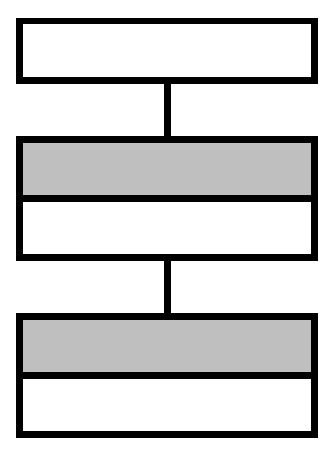
\includegraphics[scale=.15]{vcomp}
\end{minipage} \\
\rule[-2em]{0pt}{4em}
Soundness &
\rule{0pt}{5ex}
\AxiomC{$\jg{L_1}{R}{M}{L_2}$}
\UnaryInfC{$\forall P . \llbracket P \oplus M \rrbracket_{L_1} \le
		\llbracket P \rrbracket_{L_2}$}
\DisplayProof &
\tiny
\hspace{-1.5em}
$C[-] \sqsubseteq C[-]$
\end{tabular}
\end{frame}

\begin{frame}{Limitations}
  Things that work well:
  \begin{itemize}
    \item Relatively simple
    \item Explicit treatment of abstraction
    \item Moderately compositional
    \item Environment can be modelled with oracle
  \end{itemize}

  \vfill
  Things we would like to improve:
  \begin{itemize}
    \item More flexible interaction model (not just primitive calls)
    \item Interfacing with other projects
    \item Upcalls etc.
    \item Oracle is not very compositional
  \end{itemize}
\end{frame}

\begin{frame}{Solution}
  A \emph{hierarchy} of semantic models:
  \begin{itemize}
    \item keep project-specific models
      that make verification tractable;
    \item embed into more general-purpose ones
      to interface them.
  \end{itemize}

  \begin{center}
  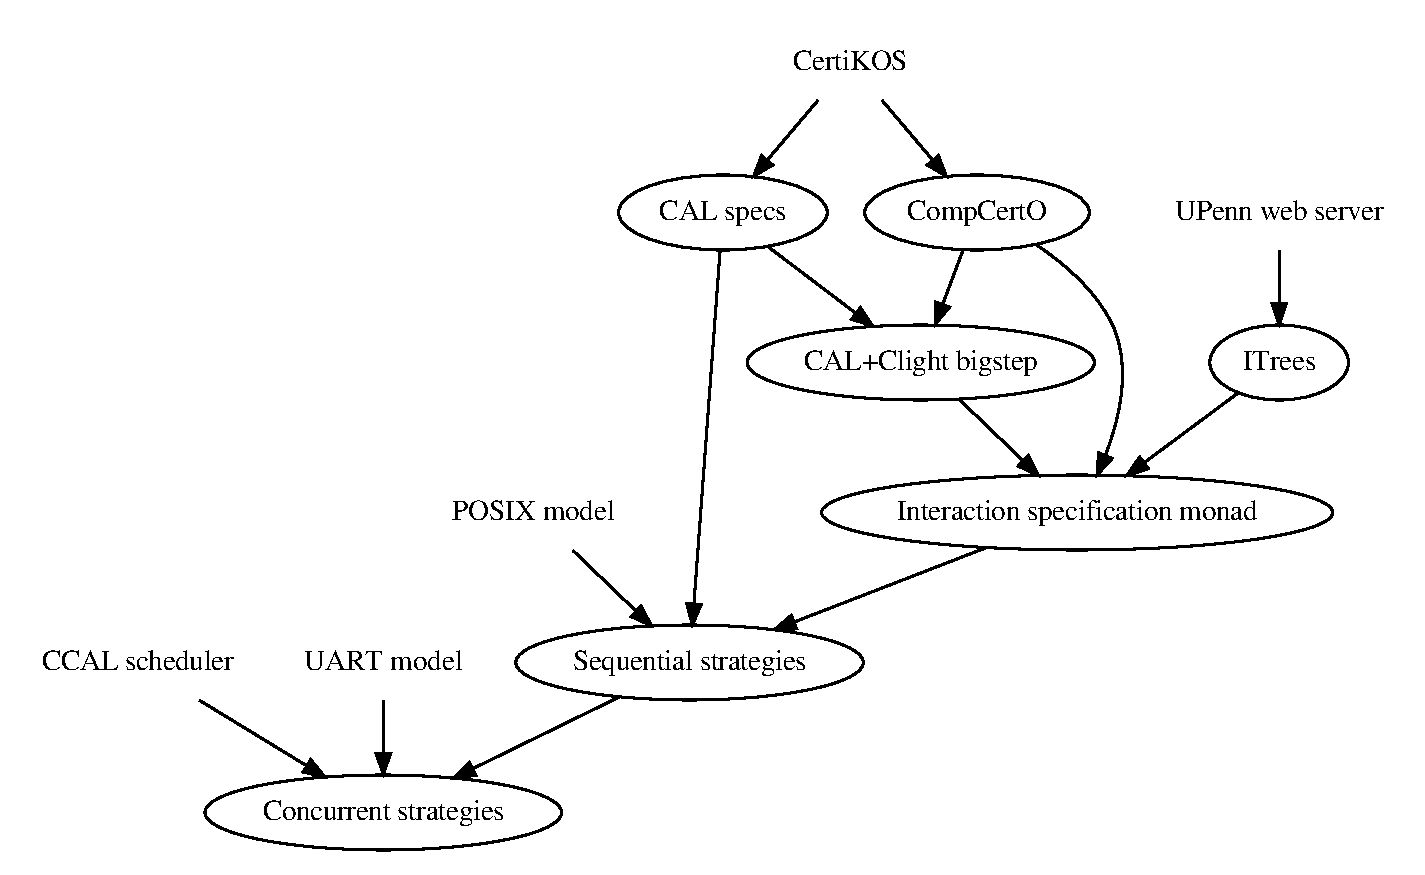
\includegraphics[scale=0.4]{hierarchy}
  \end{center}
\end{frame}

\begin{frame}{Challenge}
  What kinds of models can capture the common structures
  but adapt to particularities of each project?
\end{frame}


\section{Ingredients}

\begin{frame}{Symmetric monoidal categories}
  Symmetric monoidal categories capture structural properties
  found in many kinds of systems.
  A symmetric monoidal category has:
  \begin{itemize}
  \item Objects ($A, B$):
    type (context), layer interfaces, games, \ldots
  \item Morphisms ($f : A \rightarrow B$):
    terms, layer impl., strategies, \ldots
  \item Composition ($g \circ f$):
    substitution, vertical composition, \ldots
  \item Tensor ($A \otimes B$, $f_1 \otimes f_2$):
    pairs, horizontal composition, \ldots
  \end{itemize}

  \vfill
  This structure shows up everywhere:
  cartesian categories, abstraction layers, linear logic,
  feynman diagrams, knot theory, \ldots

  \vfill
  \textbf{Why we like it:}
  General composition algebra;
  theory is well-known and highlights connexions
  between various kinds of \emph{processes}.

  \vfill \small
  See:
  \emph{Physics, Topology, Logic and Computation: A Rosetta stone.} \\
  John C. Baez, Mike Stay.
  \url{https://arxiv.org/pdf/0903.0340.pdf}
\end{frame}

\begin{frame}{Game semantics}
  An approach to denotational semantics where:
  \begin{itemize}
    \item types are interpreted by games with players O and P;
    \item terms are interpreted by strategies ($f : A \rightarrow B$)
      which play two games simultaneously (as O in $A$, as P in $B$).
  \end{itemize}

  \vfill
  To compose the strategies $f : A \rightarrow B$ and $g : B \rightarrow C$
  into $g \circ f : A \rightarrow C$
  let them play the game $B$ against each other.

  In the tensor product
  $f_1 \otimes f_2 : A_1 \otimes A_2 \rightarrow B_1 \otimes B_2$,
  the strategies $f_1 : A_1 \rightarrow B_1$ and $f_2: A_2 \rightarrow B_2$
  play side by side.

  \vfill
  \textbf{Why we like it:}
  Games are concrete and operational,
  but can describe the behavior of all kinds of components.

  \vfill \small
  See: \emph{From CSP to Game Semantics.}
  Samson Abramsky.
  \footnotesize
  \url{https://pdfs.semanticscholar.org/72e9/762222b9ad42b5e98ebabcfc4ceca61e982b.pdf}
\end{frame}

\begin{frame}{Refinement calculus}
  In \emph{stepwise refinement} methods,
  specification constructs can be
  incrementally replaced by an executable version:
  \[
      S_1 \sqsubseteq S_2 \sqsubseteq \cdots \sqsubseteq
      S_n \sqsubseteq P \,.
  \]

  The refinement calculus allows %specifications to contain
  unbounded dual nondeterminism,
  %unbounded angelic and demonic choices.
  in the form of a lattice structure associated with $\sqsubseteq$:
%  \[
%    \begin{prooftree}
%      \hypo{P\{C_1\}Q}
%      \infer1{P\{C_1 \sqcup C_2\}Q}
%    \end{prooftree}
%    \quad
%    \begin{prooftree}
%      \hypo{P\{C_2\}Q}
%      \infer1{P\{C_1 \sqcup C_2\}Q}
%    \end{prooftree}
%    \qquad
%    \begin{prooftree}
%      \hypo{P\{C_1\}Q}
%      \hypo{P\{C_2\}Q}
%      \infer2{P\{C_1 \sqcap C_2\}Q}
%    \end{prooftree}
%  \]
  \begin{align*}
    (\forall i \in I \,.\, P_i \sqsubseteq P')
    \: &\Rightarrow \:
    \bigsqcup_{i \in I} P_i \: \sqsubseteq \: P'
    & & \text{(angelic/env. choice)}
    \\
    (\exists i \in I \,.\, P_i \sqsubseteq P')
    \: &\Rightarrow \:
    \bigsqcap_{i \in I} P_i \: \sqsubseteq \: P'
    & & \text{(demonic/system choice)}
  \end{align*}

  \textbf{Why we like it:}
  Use this to uniformly model
  not just component behaviors,
  but also specifications and correctness properties.

  \vfill
  \small
  See: \emph{Refinement calculus: a systematic introduction.}
  Back \& von Wright,
  \tiny \url{https://lara.epfl.ch/w/_media/sav08/backwright98refinementcalculus.pdf}
\end{frame}

\section{Refinement-based game semantics}

\begin{frame}{Overview}
  We will combine these ingredients into
  a series of general-purpose models.
  This week I focus on %the game model I build using
  the \emph{interaction specification monad}.

  \vfill
  Similar to interaction trees:
  \begin{itemize}
    \item \emph{Effect signatures} will provide simple games;
    \item Use a variant of the \emph{free monad} to
      describe simple strategies.
  \end{itemize}

  \vfill
  Then:
  \begin{itemize}
    \item Add a lattice structure to support specifications;
    \item Embed CAL, CompCertO, layer calculus into this model.
  \end{itemize}

  \vfill
  The monad can then be used to build a game model
  with a categorical composition algebra.
\end{frame}

\begin{frame}{Interaction specifications}
  Effect signatures specify a set of operations
  and their return type:
  \[
    E_\mathsf{bq} :=
    \{ \mathsf{enq}[v] : \mathbbm{1}, \mathsf{deq} : V \mid v \in V \}
  \]
  Then a computation with effects in $E$ and a result in $X$
  is described using plays of the form:
  \[
    m_1 n_1 \cdots m_k n_k x \,,
  \]
  where $m_i : N_i \in E$, $n_i \in N_i$, $x \in X$.

  \vfill
  The monad $\mathcal{I}_E$ adds a lattice structure.
  Operations $(m : N) \in E$ yield
  monadic operations $\mathbf{I}^m \in \mathcal{I}_E(N)$ which record events:
  \[
    \mathsf{rot} \in \mathcal{I}_{E_\mathsf{bq}}(V)
      := v \leftarrow \mathbf{I}^\mathsf{deq} ;
        \mathbf{I}^{\mathsf{enq}[v]} ; \mathsf{ret}(v)
  \]
  represents the behavior $
    \bigsqcup_{v \in V} \:
       (\mathsf{deq} \cdot v \cdot
        \mathsf{enq}[v] \cdot * \cdot v)$.
\end{frame}

\begin{frame}{Game model}
  We build a category of effect signatures
  and strategy specifications.

  For two effect signatures $E, F$,
  a morphism $f : E \rightarrow F$ is given by
  specifying an interpretation in $E$ of the operations in $F$:
  \[
    f^m \in \mathcal{I}_E(N) \qquad (m : N) \in F
  \]
  To compose $f : E \rightarrow F$ and $g : F \rightarrow G$,
  we replace the operations of $F$ used in $g$ by their
  specification in $f$:
  \[
    (g \circ f)^m := g^m[q := f^q]_{q \in F} \qquad (m \in G)
  \]
  %where $x[q := f^q]_{q \in F}$ interprets $q$ with $f^q$ so that:
  %\[
  %  \mathbf{I}^q[q := f^q]_q = f^q \qquad
  %  x[q := \mathbf{I}^q] = x
  %\]
\end{frame}

\begin{frame}{Example}
For the signatures:
\begin{align*}
  E_\mathsf{rb} &:= \{ \mathsf{set}[i,v] : \mathbbm{1},
                       \mathsf{get}[i] : V,
                       \mathsf{inc}_1 : \mathbb{N},
                       \mathsf{inc}_2 : \mathbb{N} \} \\
  E_\mathsf{bq} &:= \{ \mathsf{enq}[v] : \mathbbm{1}, \mathsf{deq} : V \} \\
  E_\mathsf{rt} &:= \{ \mathsf{rot} : V \}
\end{align*}
Consider $M : E_\mathsf{rb} \rightarrow E_\mathsf{bq}$
and $P : E_\mathsf{bq} \rightarrow E_\mathsf{rt}$:
\begin{align*}
  M^{\mathsf{enq}[v]} &:=
    i \leftarrow \mathsf{inc}_2 ; \mathsf{set}[i, v] \\
  M^{\mathsf{deq}[v]} &:=
    i \leftarrow \mathsf{inc}_1 ; \mathsf{get}[i] \\
  P^\mathsf{rot} &:= v \leftarrow \mathsf{deq} ;
    \mathsf{enq}[v] ; \mathsf{ret}(v)
\end{align*}
Then:
\begin{align*}
  (P \circ M)^\mathsf{rot} &=
    v \leftarrow (i \leftarrow \mathsf{inc}_1 ; \mathsf{get}[i]);
    (i \leftarrow \mathsf{inc}_2 ; \mathsf{set}[i, v]);
    \mathsf{ret}(v) \\
  &= i \leftarrow \mathsf{inc}_1 ; v \leftarrow \mathsf{get}[i] ;
     j \leftarrow \mathsf{inc}_2 ; \mathsf{set}[j, v] ;
     \mathsf{ret}(v)
\end{align*}
\end{frame}

\section{Conclusion}

\begin{frame}{On next week's episode \ldots}
\begin{itemize}
  \item More about dual nondeterminism
  \item CompCertO and CertiKOS
\end{itemize}
\end{frame}

\end{document}
